\documentclass[11pt]{article}
\usepackage{geometry}
\geometry{a4paper, top=20mm, left=10mm, right=10mm, bottom=20mm}
\usepackage{graphicx}
\usepackage{amsmath,amssymb,amsthm}
\usepackage{amssymb}
\usepackage[utf8]{inputenc}
\usepackage{fancyhdr}
\usepackage{lastpage}
\usepackage{enumerate}
\usepackage{enumitem}
\usepackage{multicol}
\usepackage{subcaption}
\usepackage{ifthen}
\usepackage{listings}
\usepackage{color}
\usepackage{scalerel}
\usepackage{tikz}
\usetikzlibrary{er, positioning, shapes, arrows}
%------------------------------------------ preamble
%----- fancyhdr
\fancyhead[L]{Name: Maurice Wenig}
\fancyhead[R]{Matrikelnummer: 178049}
\fancyfoot{}
\rfoot{Seite \thepage\ von \pageref{LastPage}}
\pagestyle{fancy}
%----- aufgaben
\newtheoremstyle{break}{}{5mm}{}{}{\bfseries}{}{0mm}
{\textbf{\thmname{#1}\thmnumber{ #2:} \thmnote{\textit{#3}}\newline}}
\theoremstyle{break}
\newtheorem{task}{Aufgabe}
%----- new commands
\newcommand{\Romannumeral}[1]{\MakeUppercase{\romannumeral #1}}
\newcommand{\set}[1]{\ensuremath{\{#1\}}}
\newcommand{\abs}[1]{\ensuremath{\left\vert #1 \right\vert}}
\newcommand{\norm}[1]{\ensuremath{\left\| #1 \right\|}}
\newcommand{\skal}[2]{\ensuremath{\left\langle #1 | #2 \right\rangle}}
%----- defs
\def\notiff{\mathrel{{\ooalign{\hidewidth$\not\phantom{"}$\hidewidth\cr$\iff$}}}}
\def\R{\ensuremath{\mathbb{R}}}
\def\ndy{
    \textcolor{red} {\hfill not done yet!}
    \reversemarginpar
    \marginpar{\raggedleft\textcolor{red}{\rule{2mm}{2mm}}}
}
\def\ojoin{\setbox0=\hbox{$Join$}
    \rule[0ex]{.25em}{.5pt}\llap{\rule[1.05ex]{.25em}{.5pt}}}
\def\leftouterjoin{\mathbin{\ojoin\mkern-8.5mu\Join}}
\def\fullouterjoin{\mathbin{\ojoin\mkern-8.5mu\Join\mkern-8.5mu\ojoin}}
\def\rightouterjoin{\mathbin{\Join\mkern-8.5mu\ojoin}}
%------------------------------------------ main
\begin{document}
%----- title
\begin{center}
\Large{Datenbanksysteme I}\\
\large{3. Übungsserie}
\end{center}
%----- tasks
\begin{task}
    \hfill\vspace{-5mm}
    \begin{enumerate}[label={(\alph*)}]
        \item \hfill\vspace{-5mm}\\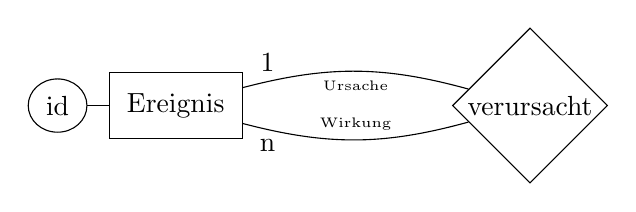
\begin{tikzpicture}[scale=3]
                \node[entity] (Ereignis) at (0.5,0) {Ereignis};
                \node[attribute] (id) at (0, 0) {id};
                \node[relationship] (verursacht) at (2,0) {verursacht};
                \draw (Ereignis) -- (id);
                \draw (Ereignis) edge[bend left=15] node[pos=0.1, above]{1} node[midway, below]{\tiny Ursache} (verursacht);
                \draw (Ereignis) edge[bend right=15] node[pos=0.1, below]{n} node[midway, above]{\tiny Wirkung} (verursacht);
            \end{tikzpicture}
        \item Ereignis(\underline{id})\\
            verursacht(Ursache, \underline{Wirkung})
        \item Ereignis(\underline{id}, Ursache)
        \item b: Ereignis $\ltimes_{\text{id=Wirkung}}$ ($\sigma$ Ursache=10 (verursacht))\\
        c: $\pi$ id ($\sigma$ Ursache=10 (Ereignis))
    \end{enumerate}
\end{task}

\begin{task}
    \hfill\vspace{-5mm}
    \begin{enumerate}[label={(\alph*)}]
        \item \begin{lstlisting}[mathescape=true]
Professoren $\ltimes$ $\rho$ PersNr$\leftarrow$gelesenVon (
    $\gamma$ gelesenVon; count(MatrNr)$\rightarrow$Anzahl (
        $\pi$ MatrNr,gelesenVon (
            $\sigma$ Semester=3 (
                Studenten$\Join$hoeren$\Join$Vorlesungen
            )
        )
    ) $\Join$ $\sigma$ Semester=3 (
        $\gamma$ Semester; count(MatrNr)$\rightarrow$Anzahl (Studenten)
    )
)
        \end{lstlisting}

        \item \begin{lstlisting}[mathescape=true]
Vorlesungen $\triangleright$ (
    $\rho$ VorlNr$\leftarrow$Nachfolger (voraussetzen)
)
        \end{lstlisting}
        
        \item \begin{lstlisting}[mathescape=true]
Profs = Professoren $\ltimes$ $\rho$ PersNr$\leftarrow$gelesenVon (
    ($\sigma$ Name='Carnap' (Studenten) $\Join$ hoeren) $\rtimes$ Vorlesung
)
Assist = Assistenten $\ltimes$ $\rho$ PName$\leftarrow$Name,Boss$\leftarrow$PersNr (Profs)
$\pi$ Name (Profs) $\cup$ $\pi$ Name (Assist)
        \end{lstlisting}
    \end{enumerate}
\end{task}

\begin{task}
    $\pi\ a,b\ (\sigma\ b\neq sb\ (R\ \times\ (\rho\ sb\leftarrow b\ (S))))$
\end{task}

\begin{task}
    \hfill\vspace{-5mm}
    \begin{enumerate}[label={(\alph*)}]
        \item $((\pi\ \text{MatrNr}\ (\text{Studenten}))\times (\pi\ \text{VorlNr}\ (\text{Vorlesungen}))) - hoeren$
        \item Studenten $\triangleright$ hoeren\\
        Studenten - (Studenten $\ltimes$ hoeren)
    \end{enumerate}
\end{task}
\end{document}